\section{Embedded Peripherals}
\begin{minipage}{0.4\linewidth}
    \subsection{Interrupts \embsys{299}{7.1}}
    \begin{itemize}
    	\item A signal indicating an event, which needs immediate CPU attention
    	\item More efficient event handling than polling
    	\item \acs{IRQ} $\rightarrow$ Interrupt Service Request
    	\item \acs{ISR} $\rightarrow$ Interrupt Service Routine
    	\item \acs{SRQ} $\rightarrow$ Service Request
    \end{itemize}
\end{minipage}
\begin{minipage}{0.5\linewidth}
    \subsubsection{Interrupt Triggers}
    \begin{tabular}{ll}
    	\textbf{Hardware Trigger}& Rising-Edge, Falling-Edge, Logic Level\\
    	\textbf{Software Trigger}& Software Event in Userprogram\\
    	\textbf{\acs{CPU} Exception}& \acs{CPU} State, Divison by Zero, Overflow etc.\\
    \end{tabular}
\end{minipage}

\subsubsection{Maskable vs Non-maskable Interrupt}
\begin{tabular}{ll}
	\textbf{Maskable Interrupt}& Can be blocked through the \acs{GIE} flag\\
	& Most commen Type of interrupt\\
	\textbf{Non-maskable Interrupt (\acs{NMI})}& Cannot be blocked, always served\\
	& Reserved for system critical events\\
\end{tabular}

\begin{minipage}{11cm}
        \subsubsection{Interrupt Identification Method \embsys{300}{7.1.1}}
    \begin{itemize}
		\item \textbf{Non-vectored Interrupt}
		\subitem Single Interrupt Line
		\subitem Single \acs{ISR} for all devices
		\subitem \acs{CPU} identifies source by polling service request (\acs{SRQ}) flags
    \end{itemize}
\end{minipage}	
	\begin{minipage}{8cm}
		\hspace{0.5cm}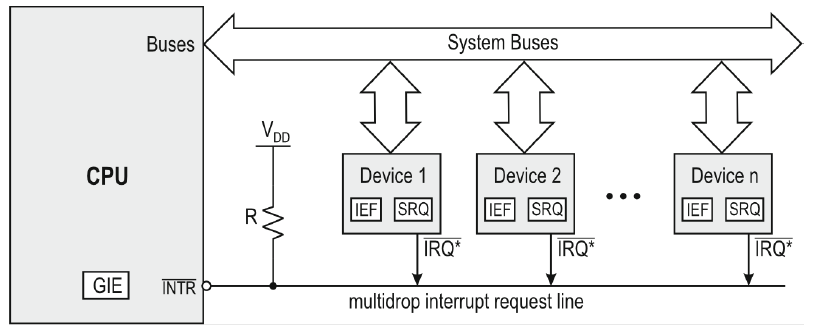
\includegraphics[width=7cm]{images/nonvectored.png}
	\end{minipage}
	\begin{minipage}{11cm}
            \begin{itemize}
		\item \textbf{Vectored Interrupt}
		\subitem Require an interrupt Acknowledgment (\acs{INTA}) cycle
		\subitem Interface generate an ID number (vector) upon \acs{INTA}
		\subitem ID Number allows calculating \acs{ISR} location
    \end{itemize}
	\end{minipage}
		\begin{minipage}{8cm}
		\hspace{0.5cm}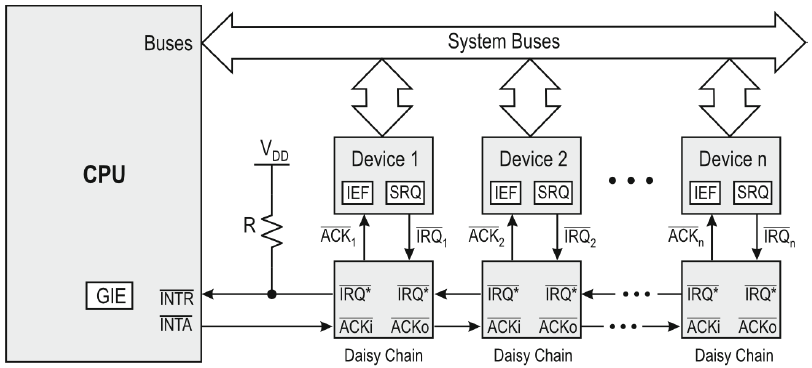
\includegraphics[width=7cm]{images/vectored.png}
	\end{minipage}
    \begin{itemize}
	\item \textbf{Auto-vectored}
	\subitem Each device has a fixed vector or \acs{ISR} adress
	\subitem No \acs{INTA} cycle or vector issuing required
	\subitem \acs{CPU} loads direct \acs{ISR} address into \acs{PC} to execute \acs{ISR}
\end{itemize}

\begin{minipage}{0.6\linewidth}
    \subsubsection{Interrupt Priority Handling \embsys{306}{7.1.5}}
    \begin{itemize}
    	\item Non-vectored Interrupt
    	\subitem Polling order of \acs{SRQ} flags decides priority
    	\item Vectored Interrupt
    	\subitem Daisy-Chain: All devices in serie. The closer the device to the \acs{CPU} the higher the priority
    	\subitem Interrupted Controlled: Uses central arbiter for resolving priorities
    \end{itemize}
\end{minipage}
\begin{minipage}{0.5\linewidth}
    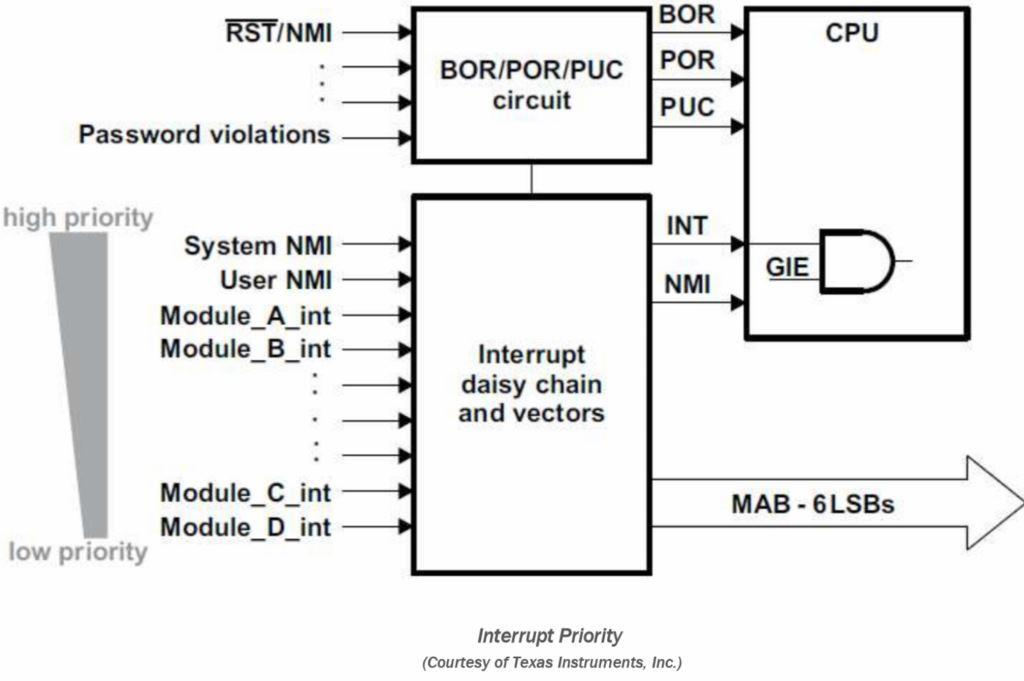
\includegraphics[width=0.9\linewidth]{images/ISRPrio}
\end{minipage}
\clearpage
\pagebreak

\subsubsection{Interrupt Service Sequence \embsys{303}{7.1.3}}
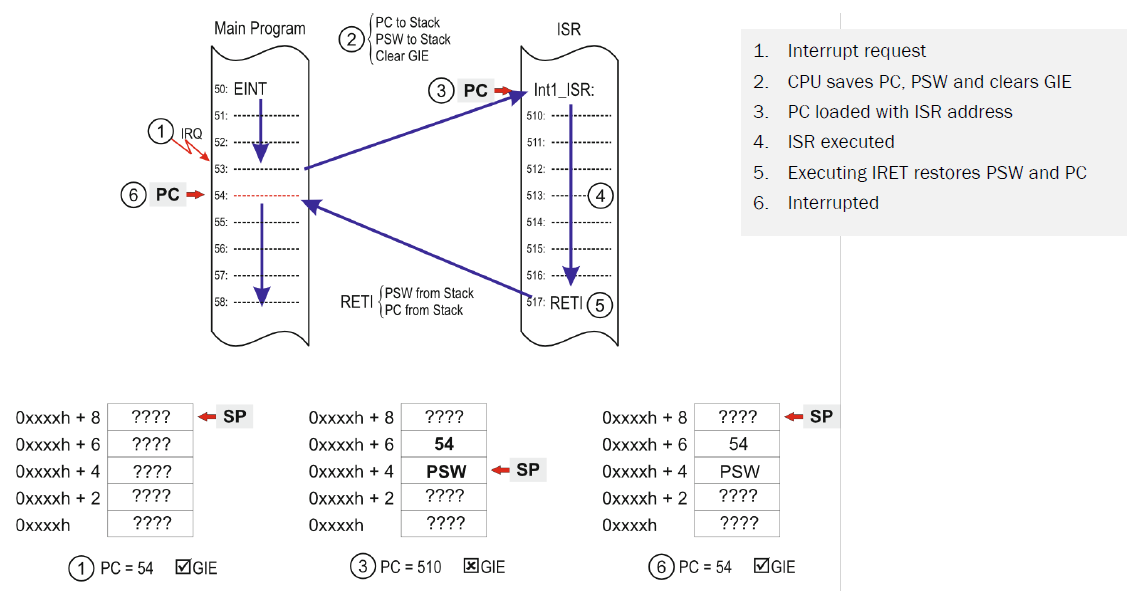
\includegraphics[width=16cm]{images/iss.png}

\subsection{Interrupthandling in the MSP430 \embsys{310}{7.2}}
\begin{itemize}
    \item Auto-vectored and Daisy-Chain
    \item System Resets: Highest priority, non-maskable, triggerd by Watchdog, Power-uP
    \item Non-maskable: Cannot be masked through \acs{GIE}-Flag, but masked through their own flag, triggerd by oscillator fault, flash key access violation
    \item Maskable: all other sources than reset \& \acs{NMI}, masked by \acs{GIE}-Flag, fixed priorities
\end{itemize}
\subsubsection{System Reset \embsys{311}{7.2.1}}
    \begin{itemize}
        \item Truly non-maskable
        \item highest system priority
        \item multisourced
        \item Saves no \acs{PC} nor \acs{PSW}
    \end{itemize}

\subsection{Interrupt Software Design \embsys{315}{7.3}}
    CodeBSP in Anhang \label{InterruptC}
    \begin{enumerate}
        \item Stack Allocation\newline
            \acs{CPU} saves \acs{SR} and \acs{PC}
        \item Vector Entry Setup\newline
            Specify entry in vector table 
        \item Interrupt Service Routine\newline
            make it Short and Quick\newline
            make Register transparent \newline
            No parameter passing or value returns\newline
            end with a \acs{RETI}
        \item Interrupt Enable\newline
            enable \acs{CPU} \acs{GIE} flag and local enables
    \end{enumerate}
\clearpage

\subsection{Timers and Event Counters \embsys{330}{7.4}}
\subsubsection{Timer Structure}
A Binary Counter Driven by a Periodic Signal. It is possible to cascade multiple counters\\
\vspace{1cm}
\begin{minipage}{0.5\linewidth}
	\begin{tabular}{ll}
		Mux           & Clock Source selector \\
		Prescaler     & Clock frequency divider \\
		Counter       & n-bit binary counter \\
		Comparator    & compares Counter Output\\
                      &  with Compare Register
	\end{tabular}
\end{minipage}
\begin{minipage}{0.5\linewidth}
	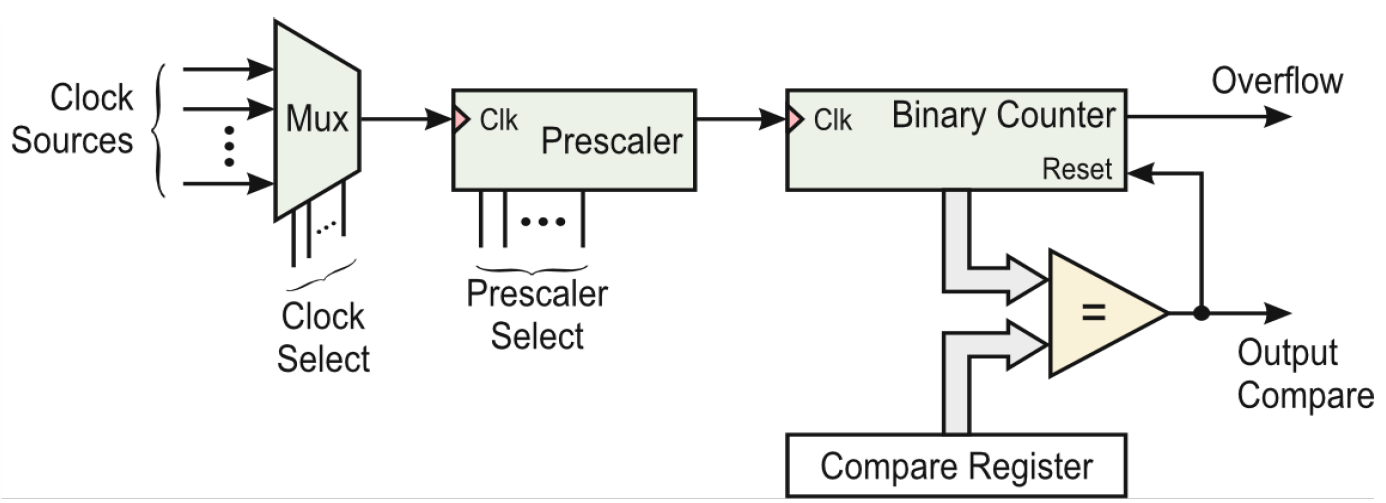
\includegraphics[width=\linewidth]{images/timerstructure.png} 
\end{minipage}
\vspace{-1.5cm}
\subsubsection{Interval Timer vs Event Counter}
	\begin{itemize}
		\item \textbf{Interval Timer}
		\subitem Measures the time elapsed after k clock cycles
		\item \textbf{Event Counter}
		\subitem Counts the occurrence of k external events
	\end{itemize}

\subsubsection{Timer Application \embsys{336}{7.4.3}}
\begin{tabular}{p{6cm} p{15cm}}
	\textbf{Watchdog Timer (\acs{WDT})} &
    Monitor Events within an expiration intervals\newline
	 If \acs{WDT} expires before the event occurs, a default action is executed\newline
	 If the event occurs within the defined interval, cancel and restart WDT\newline
	 In MSP430 the \acs{WDT} is 16-Bit (MaxCount: $2^{16}=32'768$) \newline
	 and configure over Register WDTTMSEL\\
     
	\textbf{Realtime Clocks (\acs{RTC})} &
    32-bit Timer with selectable Clock-Source\newline
    Can be used as calendar or counter (Hour.Minutes.Second)\newline
    The accuracy depend greatly on the used Cristal\\
    
	\textbf{Baud Rate Generator (\acs{BRG})} &
     $ \text{Baud Rate}=\dfrac{f_{clk}}{PS \cdot TopCount} $\newline
     PS=Prescaler Value \quad TC= Compare Value\newline
     Directly impacts Bit Time on serial communication\\
     
	\textbf{Pulse-Width Modulation (\acs{PWM})} &
    Produces a Signal which duty cycle is controlled by the \acs{MCU} \newline
    $ \text{duty cycle}=\dfrac{t_{high}}{T} $\\
\end{tabular}

\subsection{Embedded Memory Technologies \embsys{356}{7.5}}
\begin{minipage}{0.5\linewidth}
   \textbf{Control-dominated Applications}
       \begin{itemize}
       \item Program Memory
       \item Data Memory
   \end{itemize}
    \textbf{High-performance System}
\begin{itemize}
    \item Program Memory
    \item Data Memory
    \item Data Storage
\end{itemize}
\end{minipage}
\begin{minipage}{0.5\linewidth}
    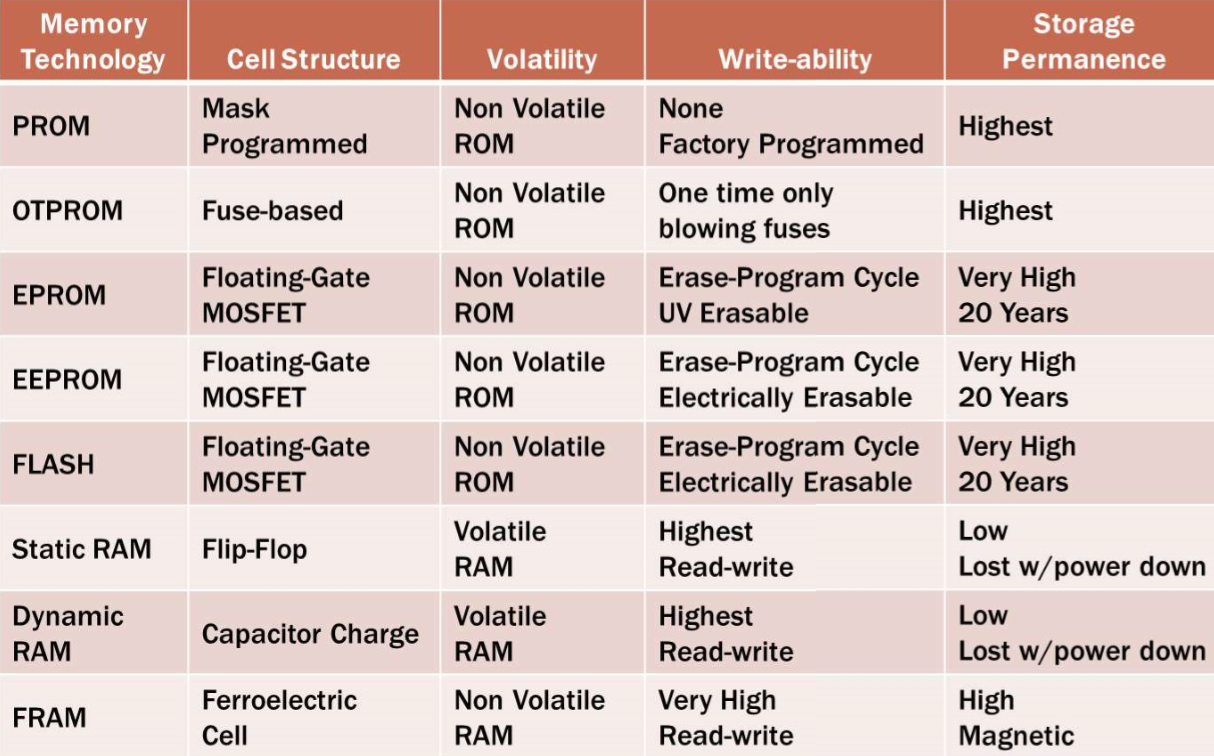
\includegraphics[width=\linewidth]{images/MemoryTech}
\end{minipage}
\clearpage
\pagebreak
%===========================================================

\subsubsection{Flash Memory and Controller \embsys{361}{7.5.3}}
\begin{minipage}{0.5\linewidth}
    \begin{itemize}
        \item Information Section
        \subitem non volatile data 
        \item Main Section
        \subitem  user programs
        \item Bootstrap Loader
        \subitem Intended for booting code 
        \subitem Contains 4 segments (A..D)
    \end{itemize}
The size of the memory depends on device and family.
\end{minipage}
\begin{minipage}{0.5\linewidth}
    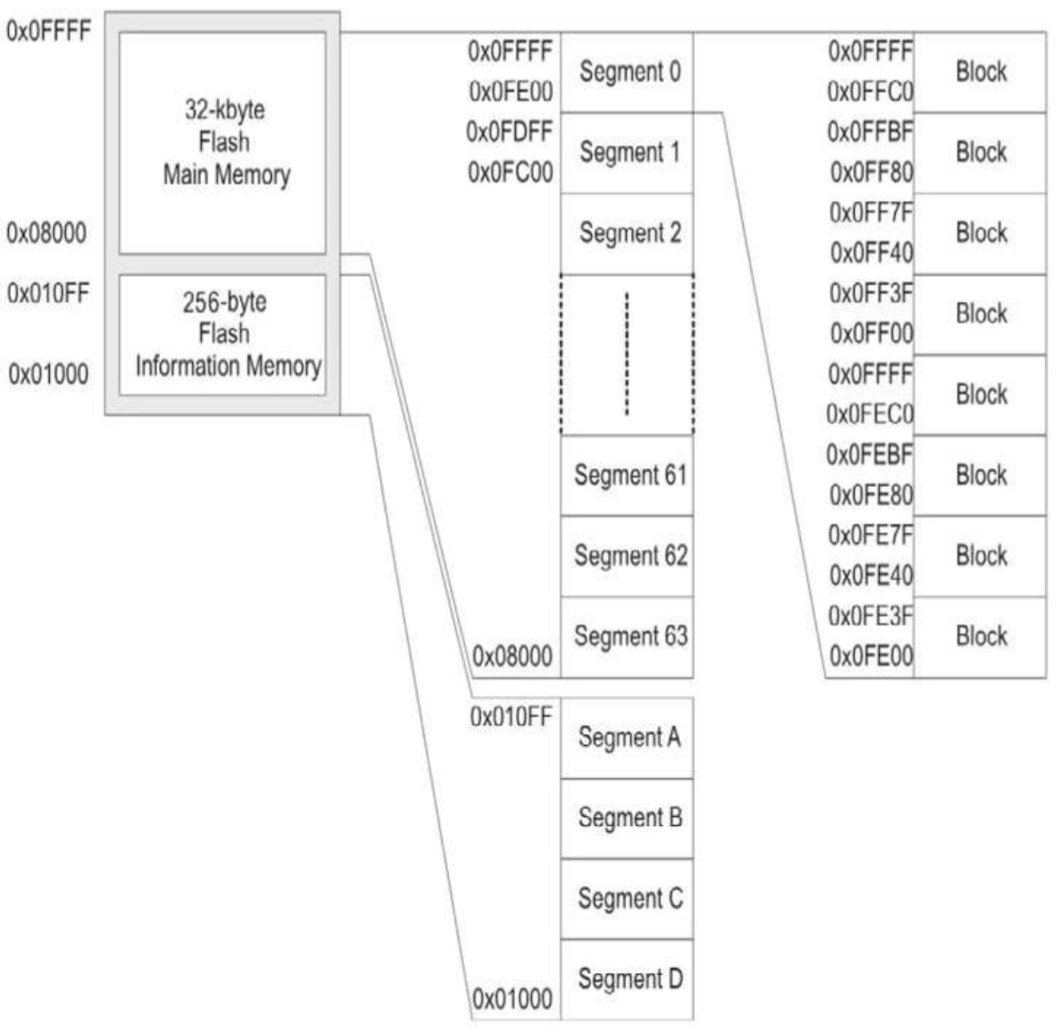
\includegraphics[width=0.7\linewidth]{images/FlashOrganization}
\end{minipage}

\subsection{Bus Arbitration and \acs{DMA} Transfers \embsys{364}{7.6}}
\begin{minipage}{0.5\linewidth}
    \subsubsection{Bus Arbitration}
    \begin{itemize}
        \item \acs{CPU} is default bus master
        \item Bus Arbitration Process
        \subitem Allows switching of the bus master
        \item Other bus master capable devices
        \subitem \acs{DMA} controllers
        \subitem \acs{GPU}
        \subitem Math Co-processor
        \subitem Other CPU's, multicore
        \item Basic Steps
        \begin{enumerate}
            \item Request
            \item Grant
            \item Release
        \end{enumerate}
    \end{itemize}
\end{minipage}
\begin{minipage}{0.5\linewidth}
    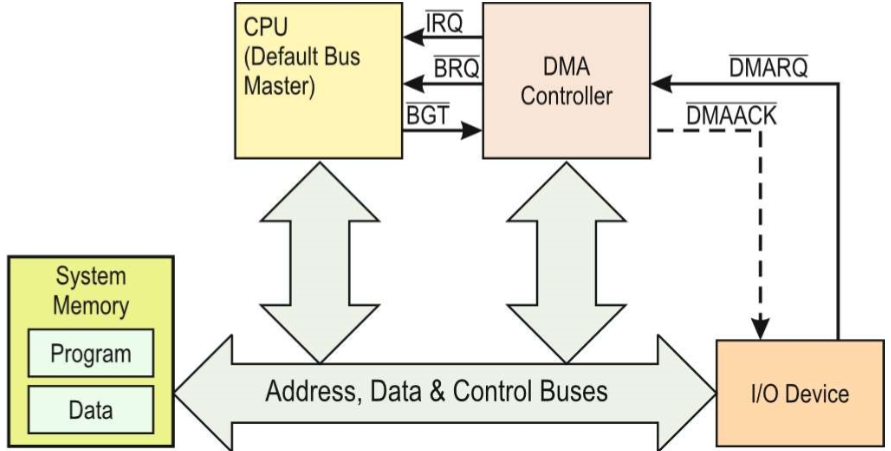
\includegraphics[width=\linewidth]{images/BusArbitrationTrans}    
    \vspace{1cm}    
    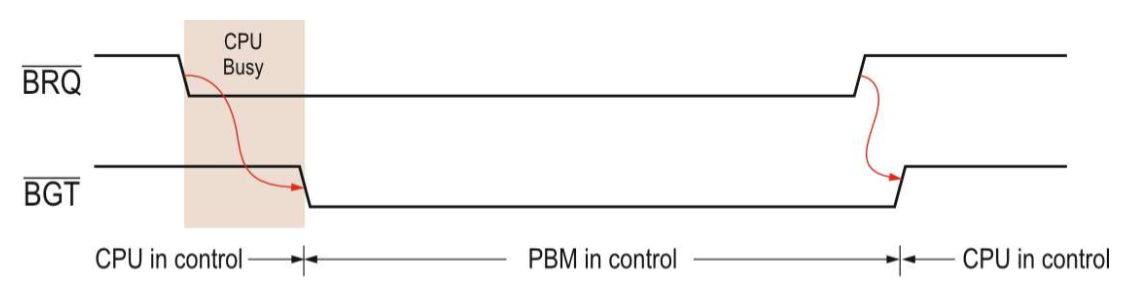
\includegraphics[width=\linewidth]{images/BusArbitrationSchem}
\end{minipage}

\subsubsection{DMA Transfers \embsys{367}{7.6.2}}
\begin{minipage}{0.8\linewidth}
       Direct Memory Access (\acs{DMA}) is a function to accelerate data transfers from peripherals.\newline
       \acs{DMA} enables direct transfer from Memory without CPU Intervention
        \begin{multicols}{2}
            \begin{minipage}{\linewidth}
                \textbf{DMA Transfer Modes}
                \begin{itemize}
                    \item Burst Mode Transfers
                        \subitem transfers entire block of data
                        \subitem for fast peripherals
                    \item Cycle Stealing Transfers
                        \subitem BAT mediates per Word
                        \subitem for slow peripherals
                    \item Transparent Transfers
                        \subitem requires additional signalisation
                        \subitem performs when \acs{CPU} is inactive
                \end{itemize}
            \end{minipage}
        
            \begin{minipage}{\linewidth}
                \textbf{\acs{DMA} Transfer Types}
                \begin{itemize}
                    \item Two-cycle \acs{DMA} Transfer
                        \subitem Data passes through
                        \subitem \acs{DMA} data register
                        \subitem S. 370
                    \item One-cycle \acs{DMA} Transfer
                        \subitem Direct \acs{I/O}-Memory path
                        \subitem S. 372
                \end{itemize}
            \end{minipage}
        \end{multicols}
\end{minipage}
\hspace{-1.5cm}
\begin{minipage}{0.2\linewidth}
    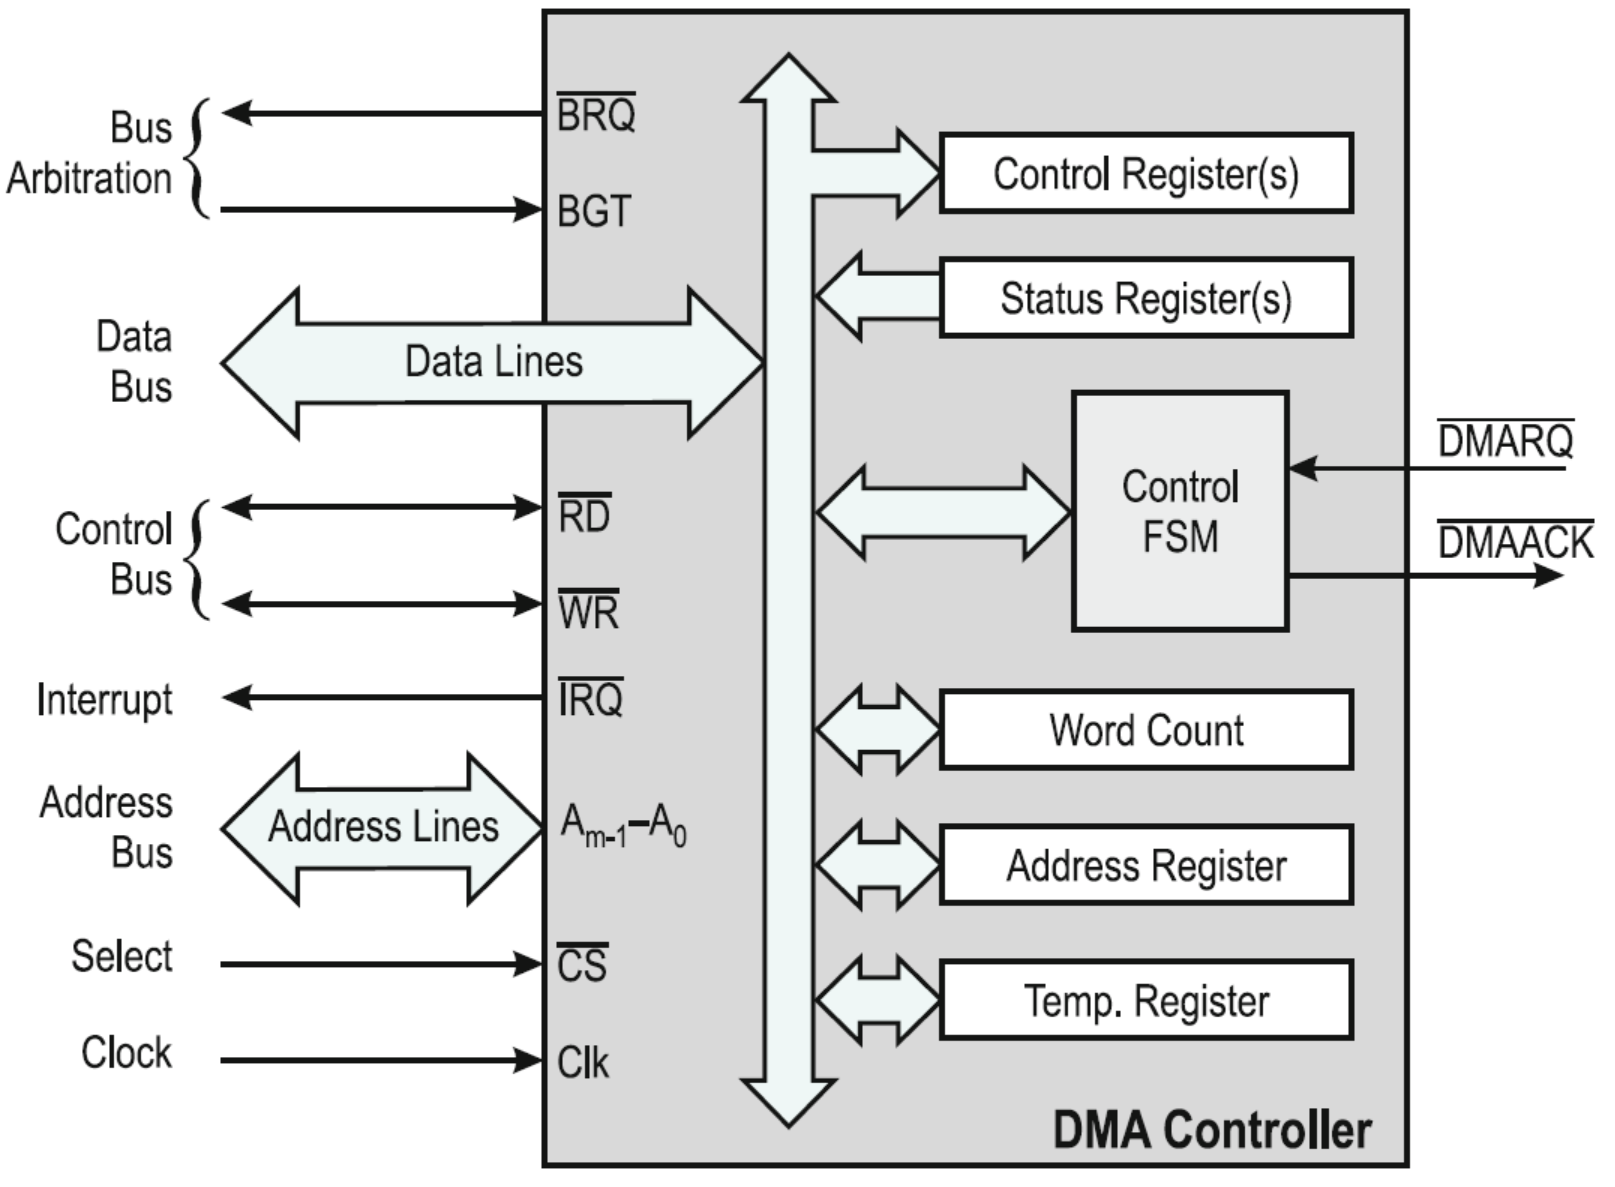
\includegraphics[width=1.5\linewidth]{images/DMAController}
\end{minipage}
    
\clearpage
\pagebreak